\listfiles
\documentclass[12pt]{report}\usepackage[]{graphicx}\usepackage[]{color}
%% maxwidth is the original width if it is less than linewidth
%% otherwise use linewidth (to make sure the graphics do not exceed the margin)
\makeatletter
\def\maxwidth{ %
  \ifdim\Gin@nat@width>\linewidth
    \linewidth
  \else
    \Gin@nat@width
  \fi
}
\makeatother

\usepackage{Sweavel}



\usepackage[intoc]{nomencl}
\textwidth=6in \oddsidemargin=0.5in \topmargin=-0.5in
\textheight=9in  % 9in must include page numbers
\textfloatsep = 0.4in 
\addtocontents{toc}{\vspace{0.4in} \protect \hfill Page\endgraf} 
\addtocontents{lof}{\vspace{0.2in} \hspace{0.13in} \ Figure \protect \hfill Page\endgraf} \addtocontents{lot}{\vspace{0.2in} \hspace{0.13in} \ Table \protect\hfill Page\endgraf}

%%%%%%%%%%%%%%%%%%%%%%%%%%%%%%%
%-------------- USE PACKAGE-----------------------------------------%
%%%%%%%%%%%%%%%%%%%%%%%%%%%%%%%

%\usepackage[natbibapa]{apacite}
\usepackage{array}
\newcolumntype{L}{>{\centering\arraybackslash}m{5cm}}
\newcolumntype{R}{>{\centering\arraybackslash}m{2cm}}

\usepackage{amsmath}
\usepackage{mathtools}
\usepackage{longtable}
\usepackage{graphicx}
\graphicspath{ {/Users/mollyolson/Documents/Vanderbilt/Masters_Thesis/ThesisRepo/} }
\usepackage{multirow}
\usepackage[font=singlespacing]{caption}
%\usepackage{caption}
%\captionsetup{font=scriptsize}
\captionsetup{font=footnotesize}
\usepackage[nottoc,notlof,notlot]{tocbibind}
\renewcommand\bibname{REFERENCES}
%\usepackage[backend=bibtex,style=verbose-trad2]{biblatex}
%\bibliography{/Users/mollyolson/Documents/Vanderbilt/Masters_Thesis/ThesisWork/thesisBib.bib}

%\usepackage{cite}


\usepackage{setspace}
\usepackage{titlesec}
\usepackage{tgschola}
\usepackage{color}
\usepackage[left=1.5in,right=1in,top=1in,bottom=1in]{geometry}
\usepackage[table]{xcolor}
 \usepackage{amsfonts}
 \usepackage{amsmath}
 \usepackage{amsbsy,bm}
 \usepackage{amssymb}
\usepackage{graphicx}
 \usepackage{setspace}
 \usepackage{rotating}
 \usepackage{float}
 \usepackage{stmaryrd}
 \usepackage{multirow}
 \usepackage{color}
 \usepackage{soul}
 \usepackage{caption}
\usepackage{eepic}
\usepackage{colortbl}
%\usepackage[numbers]{natbib}
%\usepackage{natbib}
%\usepackage{natbib}
%\setcitestyle{citesep={;}, aysep={,}}
\newcommand\harvardand{\&}

%\renewcommand{\bibname}{References}




\usepackage{multirow}
\usepackage{setspace}
\usepackage{indentfirst}
\usepackage{titlesec}
\usepackage{subfig}
\usepackage[mathscr]{euscript}
\usepackage[titletoc,title]{appendix}
\usepackage[titletoc]{appendix}
\usepackage[tocgraduated]{tocstyle}

\usepackage{textcomp}
\usepackage{array}
\usepackage{listings}
\usepackage{setspace}
\usepackage{mathptmx}
\usepackage{colortbl}
\usepackage{graphicx}
\usepackage{amssymb, amsmath}
\usepackage{subfig}
\usepackage{epsfig}
\usepackage{times}
\usepackage{float}
\usepackage{rotating}
\usepackage{makeidx}
\usepackage{url}
\usepackage{multirow}
\usepackage{booktabs}
\usepackage[subfigure, titles]{tocloft}
\usepackage[hidelinks]{hyperref}

\usepackage{acronym}
\usepackage{datetime}
\usepackage{algorithm}
\usepackage{algorithmic}
\usepackage{url, hyperref}
%\usepackage{cleveref}
\renewcommand{\nomname}{LIST OF ABBREVIATIONS}
\makenomenclature
\graphicspath{{images/}}
\DeclareGraphicsExtensions{.pdf,.jpeg,.png,.PNG, .eps, .tiff}

\urlstyle{same}

\usepackage{makecell}
\usepackage{titletoc}
\usepackage{appendix}
\usepackage[nottoc]{tocbibind}
\setcounter{secnumdepth}{7}
\setcounter{tocdepth}{7}
\usepackage{lscape}

\DeclarePairedDelimiter\ceil{\lceil}{\rceil}
\DeclarePairedDelimiter\floor{\lfloor}{\rfloor}

%%%%%%%%%%%%%%%%%%%%%%%%%%%%%%%
%-------------- NEW COMMANDS-------------------------------------%
%%%%%%%%%%%%%%%%%%%%%%%%%%%%%%%
%new chapter/section and subsection commands
\newcommand{\hsuchapter}[1]{\chapter*{#1} \addcontentsline{toc}{chapter}{#1} } 
\newcommand{\hsusection}[1]{\section*{#1} \addcontentsline{toc}{section}{#1} } 
\newcommand{\hsusubsection}[1]{\subsection*{#1} \addcontentsline{toc}{subsection}{#1} } 

%%%%%%%Configure Table of Contents%%%%%%%%%%%%
\renewcommand{\contentsname}{TABLE OF CONTENTS}
\renewcommand{\cftchapfont}{\normalfont}
\renewcommand{\cftchappagefont}{\normalfont}
\renewcommand{\cftchapleader}{\cftdotfill{\cftdotsep}}

%%%%%%%Configure List of Figures%%%%%%%%%%%%
\renewcommand{\listfigurename}{LIST OF FIGURES}
\setlength{\cftbeforefigskip}{0.2in}

%%%%%%%Configure List of Tables%%%%%%%%%%%%
\renewcommand{\listtablename}{LIST OF TABLES}
\setlength{\cftbeforetabskip}{0.2in}

%%%%%% Configure ABSTRACT %%%%%%
\usepackage{abstract}
\renewcommand{\abstractname}{ABSTRACT}




%%%%%%%Configure Bibliography%%%%%%%%%%%%
\renewcommand{\bibname}{ \texorpdfstring{{REFERENCES\vspace{10mm}}}{REFERENCES}   }

%%%%%%%%%%%%%%%%%%%%%%%%%%%%%%%
%-------------- CONFIGURE CHAPTER HEADINGS--------------%
%%%%%%%%%%%%%%%%%%%%%%%%%%%%%%%



\makeatletter
\def\@makechapterhead#1{
  {\parindent \z@ %\centering
    \LARGE \fontfamily{qcs}\selectfont
    \ifnum \c@secnumdepth >\m@ne
      \if@mainmatter
        \@chapapp\space \thechapter
        \par\nobreak
        \vskip 20\p@
      \fi
    \fi
    \interlinepenalty\@M
    #1\par\nobreak
    \vskip 40\p@
  }}
\def\@schapter#1{\if@twocolumn
                   \@topnewpage[\@makeschapterhead{#1}]%
                 \else
                   \@makeschapterhead{#1}%
                   \@afterheading
                 \fi}
\def\@makeschapterhead#1{
  {\parindent \z@ \centering
    \large
    \interlinepenalty\@M
    #1\par\nobreak
    \vskip 10\p@
  }}




%%% this configure the linespace in the table of content
%%% code is complicated and ugly but it works
\newlength{\li}\setlength{\li}{14.48pt}
\newlength{\di}\setlength{\di}{-3.5mm}
\def\@chapter[#1]#2{\ifnum \c@secnumdepth >\m@ne
      \refstepcounter{chapter}%
      \typeout{\@chapapp\space\thechapter.}%
      \addcontentsline{toc}{chapter}{\numberline{\thechapter}#1}
         %{\protect\numberline{\thechapter}\uppercase{#1}}%
      \addtocontents{toc}{\protect\vspace{\li}}%
  \else
      %\addcontentsline{toc}{chapter}{\uppercase{#1}}%
      \addcontentsline{toc}{chapter}{#1}
      \addtocontents{toc}{\protect\vspace{\li}}%
  \fi
  \chaptermark{#1}%
  \if@twocolumn
      \@topnewpage[\@makechapterhead{#2}]%
  \else
      \@makechapterhead{#2}%
      \@afterheading
 \fi}


\renewcommand\chapter{\addtocontents{toc}{\protect\addvspace{\li}}%
  \if@openright\cleardoublepage\else\clearpage\fi
  \thispagestyle{plain}%
  \global\@topnum\z@
  \@afterindentfalse
  \secdef\@chapter\@schapter}

%%%%%%%%%%%%%%%%%%%%%%%%%%%%%%%%%%%%%%%%%%%%%%%%%%%%%%%%%%%%%%
%-----------CONFIGURE SECTION HEADINGS------------------%
%%%%%%%%%%%%%%%%%%%%%%%%%%%%%%%%%%%%%%%%%%%%%%%%%%%%%%%%%%%%%%
\renewcommand\section{ \@startsection {section}{1}{\z@}%
                                   {-3.5ex \@plus -1ex \@minus -.2ex}%
                                   {2.3ex \@plus.2ex}%
                                   {\centering\large\fontfamily{qcs}\selectfont}}


                    
%%%%%%%%%%%%%%%%%%%%%%%%%%%%%%%%%%%%%%%%%%%%%%%%%%%%%%%%%%%%%%
%-------------CONFIGURE SUBSECTION HEADINGS- --------%
%%%%%%%%%%%%%%%%%%%%%%%%%%%%%%%%%%%%%%%%%%%%%%%%%%%%%%%%%%%%%%
\renewcommand\subsection{\@startsection {subsection}{2}{\z@}%
                                   {-3.5ex \@plus -1ex \@minus -.2ex}%
                                   {2.3ex \@plus.2ex}%
                                   {\noindent \large \fontfamily{qcs}\selectfont }}
                                  
      
                                   

%%%%%%%Sub-Sub-Section's Not  Supported%%%%%%%%%%%%

%%%%%%%%%%%%%%%%%%%%%%%%%%%%%%%%%%%%%%%%%%%%%%%%%%%%%%%%%%%%%%
%-------CONFIGURE TABLE OF CONTENTS HEADING------%
%%%%%%%%%%%%%%%%%%%%%%%%%%%%%%%%%%%%%%%%%%%%%%%%%%%%%%%%%%%%%%
\renewcommand{\@cftmaketoctitle}{
  \chapter*{\contentsname}
  \addcontentsline{toc}{chapter}{TABLE OF CONTENTS}} 

%%%%%%%%%%%%%%%%%%%%%%%%%%%%%%%%%%%%%%%%%%%%%%%%%%%%%%%%%%%%%%
%------CONFIGURE LIST OF FIGURES HEADING------------%
%%%%%%%%%%%%%%%%%%%%%%%%%%%%%%%%%%%%%%%%%%%%%%%%%%%%%%%%%%%%%%
\renewcommand{\@cftmakeloftitle}{
  \chapter*{\listfigurename}
  Figure \hfill Page
  \addcontentsline{toc}{chapter}{LIST OF FIGURES} } 
  
%%%%%%%%%%%%%%%%%%%%%%%%%%%%%%%%%%%%%%%%%%%%%%%%%%%%%%%%%%%%%%
%--------CONFIGURE LIST OF TABLES HEADING-------------%
%%%%%%%%%%%%%%%%%%%%%%%%%%%%%%%%%%%%%%%%%%%%%%%%%%%%%%%%%%%%%%
\renewcommand{\@cftmakelottitle}{
  \chapter*{\listtablename}
   Table \hfill Page
   \addcontentsline{toc}{chapter}{LIST OF TABLES} }  

\makeatother

\setcounter{section}{-1}     

%%%%%%%%%%%%%%%%%%%%%%%%%%%%%%%%%%%%%%%%%%%%%%%%%%%%%%%%%%%%%%
%---------------------------NEW COMMANDS-------------------------%
%%%%%%%%%%%%%%%%%%%%%%%%%%%%%%%%%%%%%%%%%%%%%%%%%%%%%%%%%%%%%%
\newcommand{\etal}{\emph{et al.}}
\newcommand{\leftsup}[2]{{\vphantom{#2}}^{#1}{#2}}
\newcommand{\leftsub}[2]{{\vphantom{#2}}_{#1}{#2}}
\newcommand{\leftsupsub}[3]{{\vphantom{#3}}^{#1}_{#2}{#3}}

\DeclareMathOperator*{\assembly}{\textbf{\Large A} }

\definecolor{lightblue}{rgb}{.90,.95,1} 
\newcommand{\hllb}[1]{
	\sethlcolor{lightblue}
	\hl{#1}
	\sethlcolor{yellow}
	}

\newcommand{\hlc}[2][yellow]{{\sethlcolor{#1}\hl{#2}} }

%%%%%%%%%%%%%%%%%%%%%%%%%%%%%%%%%%%%%%%%%%%%%%%%%%%%%%%%%%%%%%
%--------------DEFINE FLOATS----------------------------------------%
%%%%%%%%%%%%%%%%%%%%%%%%%%%%%%%%%%%%%%%%%%%%%%%%%%%%%%%%%%%%%%
 \floatstyle{plain}
 \newfloat{Box}{h}{lob}
 \newcommand{\boxedtext}[3]{
 	\begin{Box} \caption{\small{#1}}
	\hspace{1.cm}
	\fbox{\begin{minipage}[c]{0.85\linewidth} 
	
	\small{#2}
       
       \end{minipage}}
       
       \label{#3}
       \end{Box}
  }

 \begin{document}


%\pagestyle{myheadings} \markright{\today}
%%%%%%%%%%%%%%%%%%%%%%%%%%%%%%%%%%%%%%%%%%%%%%%%%%%%%%%%%%%%%%
%-------------- MAKE TITLE CHANGES HERE---------------------%
%%%%%%%%%%%%%%%%%%%%%%%%%%%%%%%%%%%%%%%%%%%%%%%%%%%%%%%%%%%%%%
\pagenumbering{alph}

\begin{titlepage}
\thispagestyle{empty}\enlargethispage{\the\footskip}%
\begin{center}
	{\setstretch{1.66} {Working Title: A Comparison of Approaches for Unplanned Sample Sizes in Phase II Clinical Trials}\par }%
	\vskip.4in
	By
	\vskip .3in
	{Molly Olson}
	\vskip .3in
	
	\begin{doublespace}
	Thesis\\
		Submitted to the Faculty of the \\
		Graduate School of Vanderbilt University \\
		in partial fulfillment of the requirements \\
		for the degree of \\ [.1in]
	\end{doublespace}
	
	\MakeUppercase{MASTER OF SCIENCE} \\[.1in]
	in \\[.1in]
	{Biostatistics} \\[.25in]
	May, 2017 \\[.25in]
	Nashville, Tennessee
	\vskip .5in
%\end{center}
%%%Uncomment for Signatures%%%
%Approved: \hskip 2.9in Date:\\[1.2em]
%\rule{3.5in}{.5pt} \hskip 0.1in \rule{2in}{.5pt} \\[.01in]
%Professor John D. Doe \\[.14in]
%\rule{3.5in}{.5pt} \hskip 0.1in \rule{2in}{.5pt}  \\[.01in]
%Professor John D. Doe \\[.14in]
%\rule{3.5in}{.5pt} \hskip 0.1in \rule{2in}{.5pt} \\[.01in]
%Professor John D. Doe \\[.14in]
%\rule{3.5in}{.5pt} \hskip 0.1in \rule{2in}{.5pt} \\[.01in]
%Professor John D. Doe \\[.14in]
%\\[.14in]
%%%%%%%%%%%%%%
%%%%%%Uncomment  for Approved Names%%%%%%
\begin{doublespace}
Approved (in progress):\\
Tatsuki Koyama , Ph.D. \\
Jeffrey Blume , Ph.D. \\
\end{doublespace}
%%%%%%%%%%%%%%%%%%%%%%%%%%%%%%%%%%%%%%%
\end{center}
\end{titlepage}
 
\doublespacing
\pagenumbering{roman} \setcounter{page}{2}

%\chapter*{The dedication page is optional. If you don't use it, please delete it.}
%\addcontentsline{toc}{chapter}{DEDICATION}
%\vspace{7mm}

%%%%%%%%%%%%%%%%%%%%%%%%%%%%%%%%%%%%%%%%%%%%%%%%%%%%%%%%%%%%%%
%--------------ACKNOWLEDGEMENTS----------- -----------------%
%%%%%%%%%%%%%%%%%%%%%%%%%%%%%%%%%%%%%%%%%%%%%%%%%%%%%%%%%%%%%%
\chapter*{ACKNOWLEDGMENTS}
\addcontentsline{toc}{chapter}{ACKNOWLEDGMENTS}
\vspace{7mm}


%%%%%%%%%%%%%%%%%%%%%%%%%%%%%%%%%%%%%%%%%%%%%%%%%%%%%%%%%%%%%%
%-------------- BEGIN TABLE OF CONTENTS---------------------%
%%%%%%%%%%%%%%%%%%%%%%%%%%%%%%%%%%%%%%%%%%%%%%%%%%%%%%%%%%%%%%
\begin{singlespace}
\tableofcontents
\newpage
\addcontentsline{toc}{chapter}{\listtablename}
\end{singlespace}

%%%%%%%%%%%%%%%%%%%%%%%%%%%%%%%%%%%%%%%%%%%%%%%%%%%%%%%%%%%%%%
%--------------BEGIN LIST OF TABLES------------------------------%
%%%%%%%%%%%%%%%%%%%%%%%%%%%%%%%%%%%%%%%%%%%%%%%%%%%%%%%%%%%%%%
\listoftables

%%%%%%%%%%%%%%%%%%%%%%%%%%%%%%%%%%%%%%%%%%%%%%%%%%%%%%%%%%%%%%
%--------------BEGIN LIST OF FIGURES----------------------------%
%%%%%%%%%%%%%%%%%%%%%%%%%%%%%%%%%%%%%%%%%%%%%%%%%%%%%%%%%%%%%%
\newpage
\addcontentsline{toc}{chapter}{\listfigurename}
\listoffigures
\newpage
%%%%%%%%%%%%%%%%%%%%%%%%%%%%%%%%%%%%%%%%%%%%%%%%%%%%%%%%%%%%%%
%-------------- ABSTRACT-----------------------------------------------%
%%%%%%%%%%%%%%%%%%%%%%%%%%%%%%%%%%%%%%%%%%%%%%%%%%%%%%%%%%%%%%
\addcontentsline{toc}{chapter}{ABSTRACT}
\chapter*{ABSTRACT}

\vspace{7mm}
Oncology phase II clinical trials are often used to evaluate the initial effect of a new regimen to determine if there is warrant further study in a phase III clinical trial. Simon's two-stage design is a commonly used design in specifying sample sizes and critical values in phase II oncology clinical trials. It is common, however, for attained sample sizes in these trials to be different than planned. In this thesis, we examine the problems in hypothesis testing for two stage phase II clinical trial designs when attained sample sizes differ from the planned design. We describe methods for redesigning trials when attained sample sizes that differ from planned and introduce a new method for redesigning a two stage clinical trial when the first stage sample sizes deviates from planned. These methods would primarily be used for prespecifying redesigns for the cases when the Simon-like design does not have planned accrual. We find that the Likelihood approach has more desireable characteristics for deviations from the planned design, though if one wishes to remain with a Frequentist approach, Olson and Koyama's method,an adaptation of a method that Chang \textit{et al.} proposed, may also be appropriate.  
\newpage

\normalsize
\doublespacing
\pagenumbering{arabic}
\setcounter{page}{1}
%%%%%%%%%%%%%%%%%%%%%%%%%%%%%%%%%%%%%%%%%%%%%%%%%%%%%%%%%%%%%%%%%%%%%%%%%%%%%%%%%%%%%%%%%%%%%%%%%%%%%%%%%%%%%%%%%%
%%%%%%%%%%%%%%%%%%%%%%%%%%%%%%%%%%%%%%%%%%%%%%%%%%%%%%%%%%%%%%%%%%%%%%%%%%%%%%%%%%%%%%%%%%%%%%%%%%%%%%%%%%%%%%%%%%
%%%%%%%%%%%%%%%%%%%%%%%%%%%%%%%%%%%%%%%%%%%%%%%%%%%%%%%%%%%%%%%%%%%%%%%%%%%%%%%%%%%%%%%%%%%%%%%%%%%%%%%%%%%%%%%%%%
%%%%%%%%%%%%%%%%%%%%%%%%%%%%%%%%%%%%%%%%%%%%%%%%%%%%%%%%%%%%%%%%%%%%%%%%%%%%%%%%%%%%%%%%%%%%%%%%%%%%%%%%%%%%%%%%%%
%% -----------------------------------WRITING STARTS HERE ------------------------------------------------------%%
%%%%%%%%%%%%%%%%%%%%%%%%%%%%%%%%%%%%%%%%%%%%%%%%%%%%%%%%%%%%%%%%%%%%%%%%%%%%%%%%%%%%%%%%%%%%%%%%%%%%%%%%%%%%%%%%%%
%%%%%%%%%%%%%%%%%%%%%%%%%%%%%%%%%%%%%%%%%%%%%%%%%%%%%%%%%%%%%%%%%%%%%%%%%%%%%%%%%%%%%%%%%%%%%%%%%%%%%%%%%%%%%%%%%%
%%%%%%%%%%%%%%%%%%%%%%%%%%%%%%%%%%%%%%%%%%%%%%%%%%%%%%%%%%%%%%%%%%%%%%%%%%%%%%%%%%%%%%%%%%%%%%%%%%%%%%%%%%%%%%%%%%
%%%%%%%%%%%%%%%%%%%%%%%%%%%%%%%%%%%%%%%%%%%%%%%%%%%%%%%%%%%%%%%%%%%%%%%%%%%%%%%%%%%%%%%%%%%%%%%%%%%%%%%%%%%%%%%%%%


%---------------------------------------------------------------------------------------------------------------%
%------------------------------------------------CHAPTER1------------------------------------------------%
%---------------------------------------------------------------------------------------------------------------%

%% comparison by itself is interesting
%% chang et al design is a little bit better - it's a new contribution so it won't feel like it's only reviews. 
%% make sure that comes out in the paper
%% maybe change the section title

%%%%%%%%%%%%%%%%%%%%%%%%%%%%%%%%%%%%%%%%%%%%%%%%%%%%%%%%%%%%%%
%------------Introduction------------------------------------%
%%%%%%%%%%%%%%%%%%%%%%%%%%%%%%%%%%%%%%%%%%%%%%%%%%%%%%%%%%%%%%
\cftlocalchange{toc}{450pt}{0cm}
\cftaddtitleline{toc}{chapter}{Chapter}{}
\cftlocalchange{toc}{1.55em}{2.55em}
\chapter{Introduction}
\vspace{-7mm}
Oncology phase II clinical trials are often used to evaluate the initial effect of a new regimen to determine if there is warrant for further study in a phase III clinical trial \cite{Porcher, Simon, Koyama}. Simon's two-stage design \cite{Simon} is a commonly used design that specifies sample sizes and critical values in phase II oncology clinical trials. Koyama and Chen \cite{Koyama} point out that it is common for actual sample sizes of these phase II trials to differ than the planned, pre-specified sample sizes. This could happen due to unanticipated accruement speed or drop-out rates and often multi-center trials can be delayed in communication of enrollment and response information. Currently, when attained sample sizes differ from planned, call these unplanned sample sizes, it is common practice to treat the attained sample sizes as planned. Though, when acheived sample sizes differ from planned, hypothesis testing using the attained sample sizes as if they were planned is not valid and hypothesis testing in these cases is not straightforward \cite{Porcher, Koyama}. Because of these reasons, extensions of Simon-like design for hypothesis testing with unplanned sample sizes is essential. \\
\indent There have been proposed Frequentist methods that handle unplanned sample sizes in the second stage while using the planned stage I sample size, but our literature review found that there were only a few Frequentist methods to handle unplanned sample sizes in stage I. Though, when focusing on deviations in sample sizes in the second stage, many proposed methods are adjusting the p-value calculation rather than proposing a redesign. Likelihood based designs, which have the ability to be an extension of Simon's design, offer a nice solution to this problem because these designs offer flexibility in sample size without inflation of type I error. Because calculations of p-values are complicated when attained sample sizes are different than planned \cite{Koyama}, we focus on methods that offer redesigns of a planned Simon-like design that will be prespecified along with the planned design.\\
\indent In this paper, we discuss the different methods for Simon's design when the attained stage II sample size is different than planned and when attained sample sizes in both stages are different than planned. We review Simon-like designs in chapter 2 and illustrate redesign methods in chapters 3 and 4. In chapter 5, we review a concrete example from a Likelihood-based clinical trial, and in chapter 6, results of a numerical and theoretical study comparing Frequentist properties of approaches in the setting where stage I sample size differs from planned are presented.    
%%%%%%%%%%%%%%%%%%%%%%%%%%%%%%%%%%%%%%%%%%%%%%%%%%%%%%%%%%%%%%
%-------------Background-------------------------------------%
%%%%%%%%%%%%%%%%%%%%%%%%%%%%%%%%%%%%%%%%%%%%%%%%%%%%%%%%%%%%%%
\chapter{Background}
\vspace{-7mm}

%------------------------------------------------------------%
%----------- Background on Simon's design -------------------%
%------------------------------------------------------------%
\indent Simon's II stage designs for clinical trials are common designs for phase II oncology clinical trials \cite{Simon}. In Simon's designs, the null hypothesis $\mbox{H}_0: p \leq p_0$ is tested against the alternative $\mbox{H}_1: p > p_1$, where $p$ is the true response probability, $p_0$ is the highest probability of response that would indicate that the research regimen is uninteresting and $p_1$ is the lowest probability of response that would indicate that the research regimen warrants further investigation. Under these hypotheses, it is required that the type I error rate remain less than $\alpha$ and power remain above $1-\beta$. The general framework of Simon's design includes a sample size and critical value in each of the two stages. Let $n_1$ denote the first stage sample size, $n_t$ the sample size at the end of the second stage, $r_1$ the first stage critical value, and $r_t$ the critical value for the end of the second stage. Let $X_1$ be the number of successes observed in the first stage and $X_2$ be the number of additional success in the second stage. In the first stage, $n_1$ patients are enrolled. If $r_1$ or fewer patients ($X_1 \leq r_1$) are successes, then the regimen is rejected and the trial is stopped for futility. If $r_1 + 1$ patients are successful, then the trial continues to the second stage. In the second stage, $n_2 = n_t - n_1$ patients are enrolled. If $r_t$ or fewer out of the $n_t$ patients are successful ($X_t = X_1 + X_2 \leq r_t$), the treatment is considered to be futile, otherwise if $r_t + 1$ patients succeed, the treatment is considered to be effective and will warrant further study.  \\

\indent Let $B$ denote the cumulative binomial distribution function and $b$ denote the binomial probability mass function. The probability of early termination with probability $p$ in Simon's designs is given by PET = $B(r_1, p, n_1)$. The expected sample size for probability $p$ is then $\mbox{EN} = n_1 + (1-\mbox{PET})n_2$, and the probability of rejecting a drug for probability $p$ is then  $$PR(p) = B(r_1, p, n_1) + \sum_{x=r_1+1}^{min[n_1,{r_t}]} b(x, p, n_1) B(r_t-x,p,n_2)$$. It is required that $PR(p) \geq 1-\alpha$ and $PR(p) \leq \beta$. Given these constraints, it follows that unconditional power, $UCP(p)$, given probability $p$, is given by 

\begin{equation*}
\begin{aligned}
1-PR(p) &= 1 - \left( B(r_1, p, n_1) + \sum_{x=r_1+1}^{min[n_1,{r_t}]} b(x, p, n_1) B(r_t-x,p,n_2) \right) \\
&= \sum_{r_1+1}^{n_1} \left\{\sum_{x_2 = r_t-x_1+1}^{n_2} b(x_2, p, n_2) \right\} b(x_1, p, n_1)
\end{aligned}
\end{equation*}
and $UCP(p_1) \geq 1-\beta$ and $UCP(p_0) \leq \alpha$. \\


\indent Simon introduced Optimal and Minimax designs. An Optimal two-stage design is a Simon's design in which minimizes the expected sample size under the null hypothesis with response value $p_0$ ($\mbox{EN}_0$) while still satisfying the type I and type II error probability restrictions. The Minimax design will minimize the maximum sample size ($n_t = n_1 + n_2$). Jung \textit{et al.} \cite{Jung} introduced an extension of Simon's designs called Admissible designs that are considered a compromise between Optimal and Minimax designs because they have similar maximim sample size as the minimax design and a similar $\mbox{EN}_0$ to the optimal design.  Admissible designs optimize a straight line on the ($n$, $EN$)-plane, $q \times n + (1-q) \times \mbox{EN}$, for some $q \in [0,1]$ \cite{Jung}. Admissible designs satisfy ($\alpha, \beta$) constraints and obtain an expected sample size somewhere between Optimal and Minimax designs. Admissible designs may be attractive because they have agreeable properties of both the Minimax and Optimal design.  Simon does not allow for early termination of the trial for efficacy \cite{Simon}, and we do not consider that design here. We focus this paper on extensions of Minimax, Optimal, and Admissible designs and call these Simon-like designs. 


%%%%%%%%%%%%%%%%%%%%%%%%%%%%%%%%%%%%%%%%%%%%%%%%%%%%%%%%%%%%%%
%------------------Literature Review-------------------------%
\chapter{Deviation from Planned Sample Sizes In Second Stage}
%%%%%%%%%%%%%%%%%%%%%%%%%%%%%%%%%%%%%%%%%%%%%%%%%%%%%%%%%%%%%%
%%%%%%%%%%%%%%%%%%%%%%%%%%%%%%%%%%%%%%%%%%%%%%%%%%%%%%%%%%%%%%%
%----------Unplanned sample size in the first stage-----------%
%\section{Deviation from Planned Sample Sizes in Second Stage}
%%%%%%%%%%%%%%%%%%%%%%%%%%%%%%%%%%%%%%%%%%%%%%%%%%%%%%%%%%%%%%%%

When over- or under-enrollment occurs, a straightforward solution is to perform an interim analysis on the planned number of first stage subjects, and adjust the testing procedure for a sample size in the second stage that is different than planned. This is possible under the assumption of non-informative dropouts; stage one is concluded when the number of non-missing patients is equal to the planned stage one sample size, and if over enrollment occurs in the first stage, they will only be considered for the second stage analysis \cite{Koyama}. Literature exists describing point estimation of the response rate and p-values for hypothesis testing when stage two sample size is modified. A review of these methods can be found by Porcher et al. \cite{Porcher}. Because Koyama and Chen have shown that the p-value in multistage trials will depend on the design and is complicated in the setting of unplanned sample sizes \cite{Koyama}, we only focus on methods that use critical values for hypothesis testing, or redesigns, and will not focus on p-value calculations. \textbf{(Basically calculating a p-value is complicated in unplanned settings, so we are just going to use critical values instead)} Koyama et al. propose a method for inference when stage II sample sizes deviate from the planned stage II sample size \cite{Koyama}. Let $n_1, n_t, r_1, r_t, \alpha$ and $\beta$ be the original design parameters. The authors let the first stage remain as planned and propose a redesign of the second stage. The authors first define conditional power, $\mbox{A}(x_1, n_2, p) = P_p[X_2 \geq r_t].$ Using conditional power evaluated at $p_0$, they calculate a new critical value, $r_t^\ast$, by finding the value of $r_t^\ast$ such that $\mbox{A}^\ast(x_1, n_2^\ast, p_0) \leq \mbox{A}(x_1, n_2, p_0) \equiv P_{p_0}[X_2^\ast \geq r_t^\ast | X_1 = x_1] \leq P_{p_0}[X_2 \geq r_t | X_1 = x_1]$, where $X_2^\ast \sim \mbox{Binomial}(n_2^\ast, p_0)$ and $n_2^\ast$ is the attained stage II sample size. This new critical value will result in a controlled unconditional type I error rate because the new critical value gives a conditional type I error rate that is more conservative than the original conditional type I error rate. The authors comment that the new critical value, $r_t^\ast$ may require a different number of total responses to reject $H_0$ for different values of $X_1$ because it is conditional on the result of the first stage. 

\newpage
%%%%%%%%%%%%%%%%%%%%%%%%%%%%%%%%%%%%%%%%%%%%%%%%%%%%%%%%%%%%%%%%
%---------Unplanned sample sizes in first stage----------------%
\chapter{Deviation from Planned Sample Sizes in First Stage}
%%%%%%%%%%%%%%%%%%%%%%%%%%%%%%%%%%%%%%%%%%%%%%%%%%%%%%%%%%%%%%%%

\indent Because accruement of patients can often be unexpected in the first stage and some situations require early evaluation of the first stage, it's imperative that methods are available to handle situations with attained sample sizes that differ from the planned sample size. Green and Dahlberg \cite{Green} and Chen and Ng \cite{Chen} propose methods for inference when first stage sample sizes differ than planned. Recall that $p_0$ is the highest probability of response that would indicate that the research regimen is uninteresting and $p_1$ is the lowest probability of response that would indicate that the research regimen warrants further investigation. Green and Dahlberg extended Southwest Oncology Group's inference method by suggesting to perform a hypothesis test on $H_0: p=p_1$ versus $H_1: p < p_1$ in the first stage at the 0.02 $\alpha$-level and concluding futility if the p-value is $\leq 0.02$. They then suggest testing $H_0: p=p_0$ versus $H_1: p < p_0$ in the second stage at the 0.05 level. Li et al. indicate that this approach controls type I error and acheives desired power, though this approach is founded on an overall $\alpha$-level of 0.05, and it is unclear how this method would generalize to any $\alpha$-level \cite{Li}. Chang et al. also point out that Green and Dahlberg's designs can possibly be quite different than the planned designed. Chen and Ng suggest an approach to unplanned sample sizes by considering a range of sample sizes in both the first and second stage. They search these ranges for the Minimax and Optimal designs that satisfy error constraints using the average probability of termination for all possible first stage sample sizes and average expected sample size for all possible stage I and stage II sample size combinations \cite{Chen}. Some limitations of this approach are that attained sample sizes may fall outside of the ranges specified, it does not consider admissible designs, and the average characteristics are only calculated rather than a specific design. Thus, we consider new approaches to unplanned sample sizes in the first stage in both the Frequentist and Likelihood settings. In the interest of prespecifying designs, we focus on deviation from the planned sample size only in the first stage. It is impractical to prespecify limitless combinations of unplanned sample sizes in both the first and second stages.   

%%%%%%%%%%%%%%%%%%%%%%%%%%%%%%%%%%%%%%%%%%%%%%%%%%%%%%%%%%%%%%
%--------------------Chang et al method----------------------%
\section{\textit{Chang et al.} Alternative Designs and Adaptation}
%%%%%%%%%%%%%%%%%%%%%%%%%%%%%%%%%%%%%%%%%%%%%%%%%%%%%%%%%%%%%%
Chang \textit{et al.} \cite{Chang} proposed an alternative design that is an extension of Simon-like two stage designs in order to handle unplanned sample sizes in both the first and second stages. This method calculates new critical values for attained sample sizes, and thus one is able to create and pre-specify a new design based on a preferred Simon or Admissible design in defense of the events of unplanned sample sizes. We use this method to pre-specify new designs; that is, we calculate new critical values for different combinations of possible deviations in sample sizes pre-attainment. Because it's desired to stay as closely to the original design as possible, we investigate this method using only attained first stage sample sizes while maintaining the original second stage sample size or original total sample size. Again, let $n_1$, $n_t$, $r_1$, $r_t$, $p_0$, $p_1$, $\alpha$, and $\beta$ be the original, planned design parameters. In the case that we let the total sample size be planned, let $n_1^{\ast \ast}$ be the attained sample size in the first stage and $n_2^{\ast\ast} = n_t - n_1^{\ast\ast}$. In the case that we let the second stage sample size remain as planned, let $n_1^{\ast\ast}$ again be the attained sample size in the first stage and $n_t^{\ast\ast} = n_2 + n_1^{\ast\ast}$. \\
\indent Chang \textit{et al.} proposes that type II error probability spent in stage I is given by $\beta_1 = \mbox{P}(X_1 \leq r_1 \vert n_1, p = p_1)$ Based on the attained sample sizes, we choose to spend type II error in the first stage established by the type II error probability spending function 
$$
\beta(m) = \left\{
        \begin{array}{ll}
            \beta_1 m/n_1 & \quad \text{if } m\leq n_1 \\
            \beta_1 + (\beta - \beta_1)(m - n_1)/n_2 & \quad \text{if } m > n_1
        \end{array}
    \right.
$$
We then find a new stage one critical value, $s_1$, using this probability spending function such that $P(X_1 \leq s_1 | n_1^{\ast\ast}) \approx \beta(n_1^{\ast\ast})$, where $\approx$ means ``closest to." After $s_1$ is selected, we then search for an integer for the second stage critical value, $s_t$, that satisfies
\begin{equation*}
\begin{aligned}
& P(X_1 > s_1, X_t > s_t | n_1^{\ast\ast}, m_2, p_0) \\
= & \sum_{s_1}^{n_1^{\ast\ast}} P(X_2 > s_t - X_1 | X_1 = x_1) P(X_1 > s_1) \\
 \leq & \alpha \\
\end{aligned}
\end{equation*}
where $m_2 = n_2$ or $n_2^{\ast\ast}$. 
Chang \textit{et al.}'s design can be used for any $\alpha$-level and is flexible, close to the original design, and preserves, on average, the desired Frequentist type I error rate. \\
%Wu \textit{et al} \cite{Wu} also proposed an adjustment to Simon’s design based on attained sample sizes in both the first and second stages. Because Wu's methods don't work very well \textbf{wording}, we won't consider their method for the remainder of this paper. 
We modify Chang \textit{et al.}'s method because we prefer to be conservative when straying from a desired Simon or Admissible design. We modify the design by selecting $s_1$ that is closest to the probability of early termination under the null, rather than using a type II error probability spending function. We select $s_1$ such that $$P(X_1 \leq s_1 | n_1^{\ast\ast}, p_0) \approx P(X_1 \leq r_1 | n_1, p_0)$$ We then select the stage two critical value, $s_t$, in the same fashion as Chang's design. Another option would be to be choose $s_1$ such that the probability of early termination with the redesign is conservative relative to the original design. In either case, the designs tend to be close when the attained sample size is close to the original, so we consider the case where the probability of early termination is closest to the original. We call this adaptation to Chang \textit{et al.}'s design ``Olson and Koyama's design"  

%------------------------------------------------------------%
%----------- Background on likelihood design ----------------%
%------------------------------------------------------------%
\section{Likelihood Design}
%\vspace{-5mm}

Briefly, the Likelihood methods use the likelihood ratio as a measure of evidence \cite{Blume}. Here, the likelihood ratio is 
\begin{equation*}
\begin{aligned}
\mbox{LR}_n & = \frac{\mbox{L}_n(p_1)}{\mbox{L}_n(p_0)} \\
&= \frac{p_1^{x_t}(1-p_1)^{n_t-x_t}}{p_0^{x_1}(1-p_0)^{n_t-x_t}} \\
& \in \left\{[0, 1/k], [1/k,k], [k, \infty)\right\}
\end{aligned}
\end{equation*}
and has three evidential zones: evidence for the null hypothesis, weak evidence, and evidence for the alternative hypothesis. If the $\mbox{LR}_n \in [0, 1/k]$, there is evidence for the null hypothesis, if $\mbox{LR}_n \in [1/k,k]$, there is weak evidence for either hypothesis, and if $\mbox{LR}_n \in [k,\infty]$, there is evidence for the alternative hypothesis. The probability of observing weak evidence is $\mbox{PW}_i = P(k_a \leq LR_n \leq k_b | H_i), k_a \leq 1 \leq k_b$, where $k_a$ and $k_b$ are benchmarks for description of evidence, the probability of observing strong evidence is 
$$
\mbox{PS}_i = \left\{
        \begin{array}{ll}
            P(LR_n > k_b|H_i) & \quad \text{if } i = 1 \\
            P(LR_n < k_b|H_i) & \quad \text{if } i = 0
        \end{array}
    \right.
$$
and the probability of obseving misleading evidence is 
$$
\mbox{PM}_i = \left\{
        \begin{array}{ll}
            P(LR_n > k_b|H_i) & \quad \text{if } i = 0 \\
            P(LR_n < k_b|H_i) & \quad \text{if } i = 1
        \end{array}
    \right.
$$
One advantage to a likelihood sequential design is that the universal bound of misleading evidence under the null hypothesis is $P(LR_n > k_b|H_0) \leq \frac{1}{k_b}$ for any $\mbox{n} \geq 1$ when $\frac{1}{k_a} = k_b = k > 1$. \\

\indent Blume and Ayers \cite{Blume} consider a phase II Likelihood two-stage design. The Likelihood two stage design will enroll $n_1$ observations into the first stage. If we observe a likelihood ratio that is $k_{a_1} < LR_{n_1} < k_{b_1}$, where $k_{a_1}$ and $k_{b_1}$ are benchmarks for description of evidence in the first stage, we continue to the second stage. If we observe $\mbox{LR}_{n_1} \leq k_{a_1}$, the study will stop for futility and if we observe $\mbox{LR}_{n_1} \geq k_{b_1}$, the study will stop for efficacy. Then, $n_2$ patients are enrolled. If the $\mbox{LR}_{n_t} = \mbox{LR}_{n_1}\mbox{LR}_{n_2}$ is $k_{a_t} < \mbox{LR}_{n_t} < k_{b_t}$, where $k_{a_t}$ and $k_{b_t}$ are benchmarks at the end of stage II, then the study will conclude with weak evidence. The study will conclude with evidence for the alternative hypothesis if $\mbox{LR}_{n_t} \geq k_{b_t}$ and evidence for the null hypothesis if $\mbox{LR}_{n_t} \leq k_{a_t}$. Because these designs are not restricted by error rates, and rather use the likelihood ratio, this method offers favorable flexibility for unplanned sample sizes in the first stage. Likewise, one is able to add cohorts and the end of the second stage when there proves to be weak evidence without penalization. \\

\indent One can adapt the Likelihood two stage design to emulate conventional, Simon-like designs such as Optimal, Minimax, or Admissible designs with binary evidential zones: reject the null or fail to reject the null. In order to do this, one can start with a Simon-like design and redesign with a likelihood ratio approach by setting
\begin{equation*}
\begin{aligned}
k_{a_1} &= \frac{p_1(1-p_0)}{p_0(1-p_1)}^{r_1} \frac{1-p_1}{1-p_0}^{n_1} = \frac{1-p_0}{1-p_1}^{r_1-n_1}\frac{p_1}{p_0}^{r_1},\\ k_{a_t}  &= \frac{p_1(1-p_0)}{p_0(1-p_1)}^{r_t} \frac{1-p_1}{1-p_0}^{n_t} = \frac{1-p_0}{1-p_1}^{r_t-n_t}\frac{p_1}{p_0}^{r_t},\\ k_{b_1} &= \infty, \\
k_{b_t} &= \infty,
\end{aligned}
\end{equation*}

where $n_1, n_t, r_1, r_2$ are Simon-like two-stage design parameters. Then, using $k_{a_j}$ and $k_{b_j}$, we recalculate the critical values, $s_1$ and $s_t$, using
\begin{equation*}
\begin{aligned}
s_1 &= \frac{log(k_{a_1}) - n_1^{\ast\ast} log(\frac{1-p_1}{1-p_0})}{log(\frac{p_1(1-p_0)}{p_0(1-p_1)})} \\
s_t &= \frac{log(k_{a_t}) - n_t log(\frac{1-p_1}{1-p_0})}{log(\frac{p_1(1-p_0)}{p_0(1-p_1)})}
\end{aligned}
\end{equation*}

If $s_1$ or $s_t$ $<$ 0, they are set equal to zero. It is possible for these critical values to be less than 0 when the study design has low sample sizes and deviation from the planned sample size is extreme. \\
\textbf{add other likelihood properties here. i.e. how to calculate p(weak), p(strong), EN, and PET}. \\

\indent Blume and Ayers describe that the Likelihood designs preserve type I error rate and are bounded by $\frac{1}{k_{b_t}}$ and are equal to $O_{p_i}\left({n}^{-1/2}\right)$. Under the likelihood design, error rates tend to be less of an issue because the the average of the error rates, $\frac{\alpha + \beta}{2}$, is minimized with the likelihood approach \cite{Blume}. For the purpose of comparing methods, we do not consider the cases in which cohorts can be added after the second stage and let the total sample size remain as planned similar to the Frequentist approach. We also only consider Likelihood redesign methods to emulate Frequentist designs -- to calculate new critical values -- and do not consider pure Likelihood method two-stage design as formerly introduced. 

% \newline
% Interim: Translating to successes. This is the region in which we move to stage 2\\
% 
% $\begin{aligned}
% & UB_{interim} = \frac{log(k_{bi}) - n_1 log(\frac{1-p_1}{1-p_0})}{log(\frac{p_1(1-p_0)}{p_0(1-p_1)})} \\
% & LB_{interim} = \frac{log(k_{ai}) - n_1 log(\frac{1-p_1}{1-p_0})}{log(\frac{p_1(1-p_0)}{p_0(1-p_1)})} \\
% &\text{(LB, UB) is the interval for weak evidence. If this was Simon's design, } LB_{interim} = r_1 \\
%   &\text{Probability of strong, misleading, and weak evidence under the null} \\
%   &\indent P(\mbox{Strong}_{0i}) = B(\floor*{LB_{interim}}, n_1, p_0) \\
%   &\indent P(Misleading_{0i}) = 1-B(\floor*{UB_{interim}}, n_1, p_0) \\
%   &\indent P(Weak_{0i}) = B(\floor*{UB_{interim}}, n_1, p_0) - B(\floor*{LB_{interim}}, n_1, p_0)\\
%   &\text{Probability of strong, misleading, and weak evidence under the alternative} \\
%   &\indent P(Strong_{0i}) = 1-B(\floor*{UB_{interim}}, n_1, p_1) \\
%   &\indent P(Misleading_{0i}) = B(\floor*{LB_{interim}}, n_1, p_1) \\
%   &\indent P(Weak_{0i}) = B(\floor*{UB_{interim}}, n_1, p_1) - B(\floor*{LB_{interim}}, n_1, p_1) \\
%   &\text{note: under Simon's, PET = 1-P(Weak)}
% \end{aligned}$
%   
%   \newpage 
% \vspace{5mm}
% \noindent \textbf{Translating likelihood properties into Simon-like design:} \\
% Final Stage: Translating to successes.\\
% $\begin{aligned}
% & \text{The amount of successes that allow for continuation to the second stage are:  }  \\                   
% & \qquad  (\floor*{LB_{interim}+1}, \floor*{min(n_1, UB_{interim})}) \\
% &\text{Probability of strong, misleading, and weak evidence under } H_p \\
% & P(Weak_p) = \sum_{x=\floor*{LB_{interim}+1}}^{\floor*{min(n_1, UB_{interim})}} \Big(b(x, n_1, p_p) \times B(UB_{interim} - x, n - n_1, p_p)\Big) - B(LB_{interim} - x, n - n_1, p_p)\\
% & P(Strong_p) = P(Strong_{0i}) + \sum_{x=\floor*{LB_{interim}+1}}^{\floor*{min(n_1, UB_{interim})}} \Big( b(x,n_1,p_0) \times B(LB_{interim} - x, n-n_1, p_0) \Big) \\
% & P(Misleading_p) = P(Misleading_{0i}) + \sum_{x=\floor*{LB_{interim}+1}}^{\floor*{min(n_1, UB_{interim})}} \Big(b(x, n_1, p_p) \times (1-B(UB_{interim} - x, n-n_1, p_p) \Big)
% \end{aligned}$
% 
% 
% \vspace{10mm}
% \noindent If we want to translate likelihood design into a Simon's design, we overwrite the LR limits above as:
% 
% $\begin{aligned}
%  &k_{ai} = OR^{r_1} \frac{1-p_1}{1-p_0}^{n_1} = \frac{1-p_0}{1-p_1}^{r_1-n_1}\frac{p_1}{p_0}^{r_1} \\
%  &k_a  = OR^{r} \frac{1-p_1}{1-p_0}^{n} = \frac{1-p_0}{1-p_1}^{r-n}\frac{p_1}{p_0}^{r}\\
%  &k_{bi} = k_b = \infty\\
% \end{aligned}$


%%%%%%%%%%%%%%%%%%%%
%% example
%%%%%%%%%%%%%%%%%%%
\chapter{Example}
In order to compare these new Frequentist and Likelihood methods for deviation of sample size in the first stage, we first introduce a concrete example. An actual phase II cancer clinical trial was designed using a Likelihood two-stage design. In order to stick to convention, the trial would only stop early for futility. The planned design parameters are $n_1 = 17$, $n_t = 41$, $r_1 = 7$, $r_t = 21$, $p_0 = 0.4$, and $p_1 = 0.6$. This study design has an expected sample size of 25.6 and a probability of early termination under the null hypothesis of 64\%. This is considered an Admissible design and meets the nominal type I error rate, $\alpha = 0.05$, and type II error rate, $\beta = 0.2$. The authors provide alternative interim stopping rules for sample sizes that deviate from the planned design using the Likelihood approach. These new designs have a probability of early termination under the null that exceed 50\% and preserve type I and type II error rates. Using the original likelihood design, but varying $n_1$, one can use Chang \textit{et al.}'s method and Olson and Koyama's method, which uses probability of early termination criteria, to obtain similar results. We keep total sample size equal to the planned total sample size in this case. We compare attained methods characteristics, in particular, type I error, power, probability of early termination under the null hypothesis, and expected sample size under the null hypothesis. We refer to the Likelihood redesign, Chang and Olson and Koyama redesigns as ``attained methods." 





\begin{table}[]
\centering
\caption{Stopping rules for deviations from first stage planned sample size concrete example}
\hspace*{-3.5cm}
\begin{tabular}{|L|R|R|R|R|L|}
\hline
Design           & $r_1$ & $n_1$ & $\mbox{PET}_0$ & $\mbox{EN}_0$ & Likelihood ratio favoring $H_0$ that corresponds to Simon's futility stopping rule \\ \hline
Likelihood       & 7     & 17    & 64\%           & 25.6          & 1/3.375                                                                            \\ \hline
Chang            & 7     & 17    & 64\%           & 25.6          &                                                                                    \\ \hline
Olson and Koyama & 7     & 17    & 64\%           & 25.6          &                                                                                    \\ \hline
Likelihood       & 8     & 19    & 67\%           & 26.3          & 1/3.375                                                                            \\ \hline
Chang            & 8     & 19    & 67\%           & 26.3          &                                                                                    \\ \hline
Olson and Koyama & 8     & 19    & 67\%           & 26.3          &                                                                                    \\ \hline
Likelihood       & 9     & 21    & 69\%           & 27.2          & 1/3.375                                                                            \\ \hline
Chang            & 9     & 21    & 69\%           & 27.2          &                                                                                    \\ \hline
Olson and Koyama & 9     & 21    & 69\%           & 27.2          &                                                                                    \\ \hline
Likelihood       & 10    & 23    & 71\%           & 28.2          & 1/3.375                                                                            \\ \hline
Chang            & 10    & 23    & 71\%           & 28.2          &                                                                                    \\ \hline
Olson and Koyama & 10    & 23    & 71\%           & 28.2          &                                                                                    \\ \hline
Likelihood       & 6     & 16    & 53\%           & 27.8          & 1/5.062                                                                            \\ \hline
Chang            & 6     & 16    & 53\%           & 27.8          &                                                                                    \\ \hline
Olson and Koyama & 7     & 16    & 72\%           & 23.1          &                                                                                    \\ \hline
Likelihood       & 7     & 18    & 56\%           & 28            & 1/5.062                                                                            \\ \hline
Chang            & 7     & 18    & 56\%           & 28            &                                                                                    \\ \hline
Olson and Koyama & 7     & 18    & 56\%           & 28            &                                                                                    \\ \hline
Likelihood       & 8     & 20    & 60\%           & 28.5          & 1/5.062                                                                            \\ \hline
Chang            & 8     & 20    & 60\%           & 28.5          &                                                                                    \\ \hline
Olson and Koyama & 8     & 20    & 60\%           & 28.5          &                                                                                    \\ \hline
\end{tabular}
\hspace*{-0.1cm}
\end{table}

This example illustrates the comprability of the three adapted design methods. Generally, the stopping rules between the Chang designs and the Likelihood design are the same when $n_1^{\ast\ast}$ ranges from 16 to 23. When $n_1 = 16$, the Olson and Koyama's design gives a more conservative critical value; this is expected by design and because of the discreteness of the binomial distribution. 


\chapter{Results}

We suggest keeping the original total planned sample size or the original planned second stage sample size the same when utilizing Chang's and Olson and Koyama's methods. We choose to keep total sample size the same in our investigation because it results in a more similar design in terms of error rates  than maintaining the original second stage sample size. Likelihood methods can result in suffering type I error, which may be a concern in this constrained setting. We also see a parabolic decrease in power in Chang's method, which isn't a fruitful result (Figure 6.1 and 6.2). We also suggest setting $n_t^{\ast\ast}=n_t$ because this inhibits the ability to stray extremely far from the planned design. If one employs Chang's method, is radical in the first stage, and the resulting probability of continuing is less than 0.05, it will be impossible to make a type I error. This will then reduce the two-stage design to a one-stage design.    





\begin{figure}[]
\caption{Monte Carlo Simulation of Average Power of 20 Simon-like Designs when Stage I Sample Size Deviates from Planned for Attained Designs ($n_t^{\ast\ast} = n_1^{\ast\ast} + n_2$). Number of Simulations = 500.}
\centering
\begin{Schunk}


\centerline{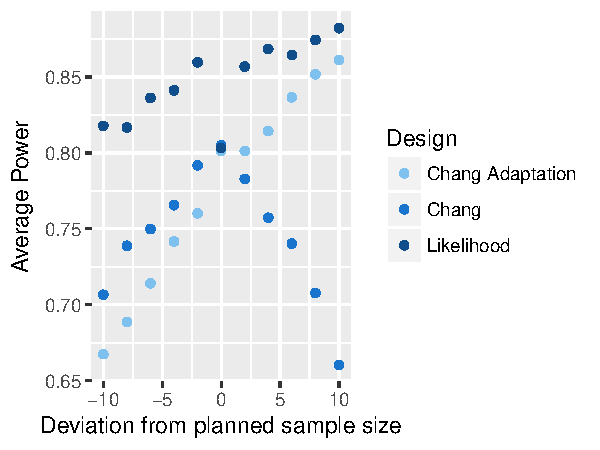
\includegraphics{unnamed-chunk-5-1} }

\end{Schunk}
\end{figure}
\begin{figure}[]
\caption{Monte Carlo Simulation of Average Power of 20 Simon-like Designs when Stage I Sample Size Deviates from Planned for Attained Designs ($n_t^{\ast\ast} = n_1^{\ast\ast} + n_2$) Number of Simulations = 500.}
\centering
\begin{Schunk}


\centerline{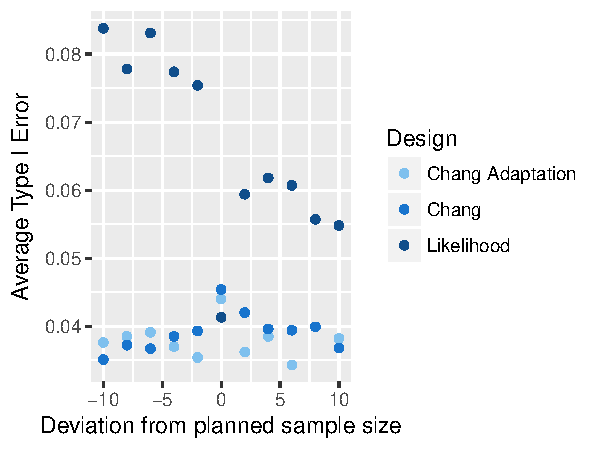
\includegraphics{unnamed-chunk-6-1} }

\end{Schunk}
\end{figure}
\indent We present results that are limited to our primary problem of interest in Tables 6.1 through 6.6. In each design table, the planned design is specified and the first stage sample size varies from planned, while maintaining the original total sample size. We compare attained methods characteristics, in particular, type I error, power, probability of early termination under the null hypothesis, and expected sample size under the null hypothesis. We refer to the Likelihood redesign, Chang and adaptation to Chang redesigns as ``attained methods." \\
\indent Table 6.1 displays a planned Admissible design with varying first stage sample size $\pm$ 10. We notice that under low $p_0$ and $p_1$, $s_1$ will vary between each method. Though, power and type I error are likely to be similar between and within each attained method, and expected sample size is also consistent. The Likelihood and Chang method are at risk of low probability of early termination, especially when the sample size is lower than planned. Table 6.2 shows an Optimal design when $p_0$ is 0.5. Between attained designs, particularly when there is overaccrual, $s_1$ is inconsistent. We particularly see a large difference when $n_1^{\ast\ast} = n_1 + 10$ between the Likelihood and Olson and Koyama designs and the Chang design.  The Likelihood design is anticonservative in type I error and conservative in type II error here, displaying a $\alpha^{\ast\ast} > \alpha$ and $1-\beta^{\ast\ast} > 1-\beta$. The Chang designs both have a conservative type I error for all sample size deviations, though Chang and Likelihood designs maintain higher power than Olson and Koyama's. Probability of early termination is closest to the original under Olson and Koyama's, and thus have a much lower expected sample size under the null hypothesis, with as much as a difference of approximately 23.\\
\indent Table 6.3 displays results from a planned Minimax design when $p_0$ is larger than 0.5. Here, the Likelihood design has desireable properties with type I error and power consistently closed to the planned design for all deviations in sample size. Though, when the sample size is severely underaccrued, the probability of early termination nearly halves. The expected sample size is consistent between designs. The Chang designs stray from the planned nominal type I and type II errors when there is overaccrual. The $\mbox{PET}_0$ for the original Chang design varies significantly between deviations. \\
\indent Table 6.4 through 6.6 display results for planned designs when $\alpha = \beta = 0.1$. Table 6.4 displays attained design characteristics for deviations in sample size when the planned first stage sample size is low. In all three attained designs, we see that as the attained sample size is lower than planned, there is a significant drop in power and a moderate to severe drop in type I error. The probability of early termination almost occurs with probability 1 when the attained sample size is $n_1^{\ast\ast} = 1$. In practice, though, accrual lower than planned here is not practical. When there is overaccrual, attained design characteristics are not concerning. \\
\indent Table 6.5 illustrates the similarity between attained designs when $p_0$ = 0.3. All designs and their deviations are relatively consistent in type I error, power, and $\mbox{PET}_0$. Though, the Olson and Koyama's design is most consistent in the probability of early termination with the planned design, but we see a conservative deviation in type I error for large overaccrual. Table 6.6 displays similar results as Table 5.3. \\




\begin{landscape}

%%%%%%%%%%%%%%%%%%%%%%
%% Table 1
%%%%%%%%%%%%%%%%%%%%%%
\begin{table}[]
\caption{Attained design characteristics from deviation of Admissible II stage design ($p_0$ = 0.1, $p_1$ = 0.25, $\alpha$ = 0.05, $\beta$ = 0.20)}
\small
  \resizebox{\columnwidth}{!}{%

\begin{tabular}{ccccccccccccccccccccccccccc}
  \hline
    \multicolumn{7}{c}{Planned Design}&\multicolumn{3}{r}{Attained Sample Size}&\multicolumn{8}{r}{Redesign}\\
  \multicolumn{8}{c}{     }&\multicolumn{1}{l}{  }&\multicolumn{6}{l}{Chang Design}&\multicolumn{6}{l}{Olson and Koyama Design}&\multicolumn{6}{l}{Likelihood Design}\\
$p_0$ & $p_1$ & $n_1$ & $n$ & $r_1$ & $r_t$ & $\mbox{PET}_0$ &$\mbox{EN}_0$ & $n_1^{\ast\ast}$ & $s_1$ & $s_t$ & $\alpha^{\ast\ast}$ & $1-\beta^{\ast\ast}$ & $\mbox{PET}_0^{\ast\ast}$ & $\mbox{EN}_0^{\ast\ast}$ & $s_1$ & $s_t$ & $\alpha^{\ast\ast}$ & $1-\beta^{\ast\ast}$ & $\mbox{PET}_0^{\ast\ast}$ & $\mbox{EN}_0^{\ast\ast}$ & $s_1$ & $s_t$ & $\alpha^{\ast\ast}$ & $1-\beta^{\ast\ast}$ & $\mbox{PET}_0^{\ast\ast}$ & $\mbox{EN}_0^{\ast\ast}$ \\ 
  \hline
0.1 & 0.25 & 15 & 41 & 1 & 7 & 0.549 & 26.725 & 5 & 0 & 7 & 0.034 & 0.671 & 0.590 & 19.742 & 0 & 7 & 0.034 & 0.671 & 0.590 & 19.742 & 0 & 7 & 0.034 & 0.671 & 0.590 & 19.742 \\ 
  0.1 & 0.25 & 15 & 41 & 1 & 7 & 0.549 & 26.725 & 7 & 0 & 7 & 0.040 & 0.754 & 0.478 & 24.738 & 0 & 7 & 0.040 & 0.754 & 0.478 & 24.738 & 0 & 7 & 0.040 & 0.754 & 0.478 & 24.738 \\ 
  0.1 & 0.25 & 15 & 41 & 1 & 7 & 0.549 & 26.725 & 9 & 0 & 7 & 0.043 & 0.797 & 0.387 & 28.603 & 0 & 7 & 0.043 & 0.797 & 0.387 & 28.603 & 0 & 7 & 0.043 & 0.797 & 0.387 & 28.603 \\ 
  0.1 & 0.25 & 15 & 41 & 1 & 7 & 0.549 & 26.725 & 11 & 0 & 7 & 0.045 & 0.819 & 0.314 & 31.586 & 1 & 7 & 0.035 & 0.718 & 0.697 & 20.079 & 0 & 7 & 0.045 & 0.819 & 0.314 & 31.586 \\ 
  0.1 & 0.25 & 15 & 41 & 1 & 7 & 0.549 & 26.725 & 13 & 0 & 7 & 0.046 & 0.830 & 0.254 & 33.883 & 1 & 7 & 0.040 & 0.771 & 0.621 & 23.602 & 0 & 7 & 0.046 & 0.830 & 0.254 & 33.883 \\ 
  0.1 & 0.25 & 15 & 41 & 1 & 7 & 0.549 & 26.725 & 15 & 1 & 7 & 0.043 & 0.803 & 0.549 & 26.725 & 1 & 7 & 0.043 & 0.803 & 0.549 & 26.725 & 1 & 7 & 0.043 & 0.803 & 0.549 & 26.725 \\ 
  0.1 & 0.25 & 15 & 41 & 1 & 7 & 0.549 & 26.725 & 17 & 1 & 7 & 0.045 & 0.821 & 0.482 & 29.437 & 1 & 7 & 0.045 & 0.821 & 0.482 & 29.437 & 1 & 7 & 0.045 & 0.821 & 0.482 & 29.437 \\ 
  0.1 & 0.25 & 15 & 41 & 1 & 7 & 0.549 & 26.725 & 19 & 2 & 7 & 0.041 & 0.792 & 0.705 & 25.480 & 1 & 7 & 0.046 & 0.831 & 0.420 & 31.754 & 1 & 7 & 0.046 & 0.831 & 0.420 & 31.754 \\ 
  0.1 & 0.25 & 15 & 41 & 1 & 7 & 0.549 & 26.725 & 21 & 2 & 7 & 0.044 & 0.814 & 0.648 & 28.032 & 2 & 7 & 0.044 & 0.814 & 0.648 & 28.032 & 1 & 7 & 0.047 & 0.836 & 0.365 & 33.705 \\ 
  0.1 & 0.25 & 15 & 41 & 1 & 7 & 0.549 & 26.725 & 23 & 3 & 7 & 0.040 & 0.785 & 0.807 & 26.469 & 2 & 7 & 0.046 & 0.827 & 0.592 & 30.345 & 2 & 7 & 0.046 & 0.827 & 0.592 & 30.345 \\ 
  0.1 & 0.25 & 15 & 41 & 1 & 7 & 0.549 & 26.725 & 25 & 3 & 7 & 0.043 & 0.810 & 0.764 & 28.783 & 2 & 7 & 0.047 & 0.834 & 0.537 & 32.406 & 2 & 7 & 0.047 & 0.834 & 0.537 & 32.406 \\ 
   \hline
\end{tabular}
}
\end{table}

%%%%%%%%%%%%%%%%%%%%%%
%% Table 2
%%%%%%%%%%%%%%%%%%%%%%
\begin{table}[]
\caption{Attained design characteristics from deviation of Simon's Optimal II stage design ($p_0$ = 0.5, $p_1$ = 0.65, $\alpha$ = 0.05, $\beta$ = 0.2)}
\small
  \resizebox{\columnwidth}{!}{%

\begin{tabular}{ccccccccccccccccccccccccccc}
  \hline
    \multicolumn{7}{c}{Planned Design}&\multicolumn{3}{r}{Attained Sample Size}&\multicolumn{8}{r}{Redesign}\\
  \multicolumn{8}{c}{     }&\multicolumn{1}{l}{  }&\multicolumn{6}{l}{Chang Design}&\multicolumn{6}{l}{Olson and Koyama Design}&\multicolumn{6}{l}{Likelihood Design}\\
$p_0$ & $p_1$ & $n_1$ & $n$ & $r_1$ & $r_t$ & $\mbox{PET}_0$ &$\mbox{EN}_0$ & $n_1^{\ast\ast}$ & $s_1$ & $s_t$ & $\alpha^{\ast\ast}$ & $1-\beta^{\ast\ast}$ & $\mbox{PET}_0^{\ast\ast}$ & $\mbox{EN}_0^{\ast\ast}$ & $s_1$ & $s_t$ & $\alpha^{\ast\ast}$ & $1-\beta^{\ast\ast}$ & $\mbox{PET}_0^{\ast\ast}$ & $\mbox{EN}_0^{\ast\ast}$ & $s_1$ & $s_t$ & $\alpha^{\ast\ast}$ & $1-\beta^{\ast\ast}$ & $\mbox{PET}_0^{\ast\ast}$ & $\mbox{EN}_0^{\ast\ast}$ \\ 
  \hline
0.5 & 0.65 & 28 & 83 & 15 & 48 & 0.714 & 43.719 & 18 & 8 & 49 & 0.036 & 0.815 & 0.407 & 56.528 & 10 & 48 & 0.037 & 0.685 & 0.760 & 33.622 & 9 & 48 & 0.048 & 0.796 & 0.593 & 44.472 \\ 
  0.5 & 0.65 & 28 & 83 & 15 & 48 & 0.714 & 43.719 & 20 & 10 & 48 & 0.050 & 0.811 & 0.588 & 45.950 & 11 & 48 & 0.039 & 0.716 & 0.748 & 35.859 & 10 & 48 & 0.050 & 0.811 & 0.588 & 45.950 \\ 
  0.5 & 0.65 & 28 & 83 & 15 & 48 & 0.714 & 43.719 & 22 & 11 & 49 & 0.034 & 0.788 & 0.584 & 47.370 & 12 & 48 & 0.042 & 0.743 & 0.738 & 37.966 & 11 & 48 & 0.051 & 0.824 & 0.584 & 47.370 \\ 
  0.5 & 0.65 & 28 & 83 & 15 & 48 & 0.714 & 43.719 & 24 & 12 & 49 & 0.034 & 0.798 & 0.581 & 48.745 & 13 & 48 & 0.044 & 0.765 & 0.729 & 39.967 & 12 & 48 & 0.052 & 0.835 & 0.581 & 48.745 \\ 
  0.5 & 0.65 & 28 & 83 & 15 & 48 & 0.714 & 43.719 & 26 & 14 & 48 & 0.045 & 0.785 & 0.721 & 41.880 & 14 & 48 & 0.045 & 0.785 & 0.721 & 41.880 & 13 & 48 & 0.053 & 0.845 & 0.577 & 50.083 \\ 
  0.5 & 0.65 & 28 & 83 & 15 & 48 & 0.714 & 43.719 & 28 & 15 & 48 & 0.047 & 0.802 & 0.714 & 43.719 & 15 & 48 & 0.047 & 0.802 & 0.714 & 43.719 & 15 & 48 & 0.047 & 0.802 & 0.714 & 43.719 \\ 
  0.5 & 0.65 & 28 & 83 & 15 & 48 & 0.714 & 43.719 & 30 & 16 & 48 & 0.049 & 0.816 & 0.708 & 45.494 & 16 & 48 & 0.049 & 0.816 & 0.708 & 45.494 & 16 & 48 & 0.049 & 0.816 & 0.708 & 45.494 \\ 
  0.5 & 0.65 & 28 & 83 & 15 & 48 & 0.714 & 43.719 & 32 & 17 & 49 & 0.033 & 0.793 & 0.702 & 47.214 & 17 & 49 & 0.033 & 0.793 & 0.702 & 47.214 & 17 & 48 & 0.050 & 0.828 & 0.702 & 47.214 \\ 
  0.5 & 0.65 & 28 & 83 & 15 & 48 & 0.714 & 43.719 & 34 & 19 & 48 & 0.043 & 0.782 & 0.804 & 43.592 & 18 & 49 & 0.034 & 0.803 & 0.696 & 48.886 & 18 & 48 & 0.051 & 0.839 & 0.696 & 48.886 \\ 
  0.5 & 0.65 & 28 & 83 & 15 & 48 & 0.714 & 43.719 & 36 & 20 & 48 & 0.045 & 0.798 & 0.797 & 45.518 & 19 & 49 & 0.035 & 0.811 & 0.691 & 50.516 & 19 & 48 & 0.053 & 0.848 & 0.691 & 50.516 \\ 
  0.5 & 0.65 & 28 & 83 & 15 & 48 & 0.714 & 43.719 & 38 & 21 & 48 & 0.047 & 0.813 & 0.791 & 47.398 & 20 & 49 & 0.035 & 0.818 & 0.686 & 52.110 & 20 & 48 & 0.054 & 0.856 & 0.686 & 52.110 \\
   \hline
\end{tabular}
}
\end{table}

%%%%%%%%%%%%%%%%%%%%%%
%% Table 3
%%%%%%%%%%%%%%%%%%%%%%
\begin{table}[]
\caption{Attained design characteristics from deviation of Simon's Minimax II stage design ($p_0$ = 0.75, $p_1$ = 0.9, $\alpha$ = 0.05, $\beta$ = 0.2)}
\small
  \resizebox{\columnwidth}{!}{%

\begin{tabular}{ccccccccccccccccccccccccccc}
  \hline
    \multicolumn{7}{c}{Planned Design}&\multicolumn{3}{r}{Attained Sample Size}&\multicolumn{8}{r}{Redesign}\\
  \multicolumn{8}{c}{     }&\multicolumn{1}{l}{  }&\multicolumn{6}{l}{Chang Design}&\multicolumn{6}{l}{Olson and Koyama Design}&\multicolumn{6}{l}{Likelihood Design}\\
$p_0$ & $p_1$ & $n_1$ & $n$ & $r_1$ & $r_t$ & $\mbox{PET}_0$ &$\mbox{EN}_0$ & $n_1^{\ast\ast}$ & $s_1$ & $s_t$ & $\alpha^{\ast\ast}$ & $1-\beta^{\ast\ast}$ & $\mbox{PET}_0^{\ast\ast}$ & $\mbox{EN}_0^{\ast\ast}$ & $s_1$ & $s_t$ & $\alpha^{\ast\ast}$ & $1-\beta^{\ast\ast}$ & $\mbox{PET}_0^{\ast\ast}$ & $\mbox{EN}_0^{\ast\ast}$ & $s_1$ & $s_t$ & $\alpha^{\ast\ast}$ & $1-\beta^{\ast\ast}$ & $\mbox{PET}_0^{\ast\ast}$ & $\mbox{EN}_0^{\ast\ast}$ \\ 
  \hline
0.75 & 0.9 & 22 & 39 & 17 & 33 & 0.677 & 27.499 & 12 & 8 & 34 & 0.019 & 0.648 & 0.351 & 29.517 & 9 & 33 & 0.045 & 0.763 & 0.609 & 22.548 & 8 & 33 & 0.050 & 0.805 & 0.351 & 29.517 \\ 
  0.75 & 0.9 & 22 & 39 & 17 & 33 & 0.677 & 27.499 & 14 & 10 & 33 & 0.050 & 0.800 & 0.479 & 27.033 & 11 & 33 & 0.042 & 0.738 & 0.719 & 21.028 & 10 & 33 & 0.050 & 0.800 & 0.479 & 27.033 \\ 
  0.75 & 0.9 & 22 & 39 & 17 & 33 & 0.677 & 27.499 & 16 & 12 & 33 & 0.048 & 0.792 & 0.595 & 25.315 & 12 & 33 & 0.048 & 0.792 & 0.595 & 25.315 & 11 & 33 & 0.051 & 0.809 & 0.370 & 30.494 \\ 
  0.75 & 0.9 & 22 & 39 & 17 & 33 & 0.677 & 27.499 & 18 & 13 & 34 & 0.019 & 0.650 & 0.481 & 28.892 & 14 & 33 & 0.047 & 0.782 & 0.694 & 24.419 & 13 & 33 & 0.051 & 0.807 & 0.481 & 28.892 \\ 
  0.75 & 0.9 & 22 & 39 & 17 & 33 & 0.677 & 27.499 & 20 & 15 & 34 & 0.019 & 0.650 & 0.585 & 27.882 & 15 & 34 & 0.019 & 0.650 & 0.585 & 27.882 & 15 & 33 & 0.050 & 0.805 & 0.585 & 27.882 \\ 
  0.75 & 0.9 & 22 & 39 & 17 & 33 & 0.677 & 27.499 & 22 & 17 & 33 & 0.050 & 0.802 & 0.677 & 27.499 & 17 & 33 & 0.050 & 0.802 & 0.677 & 27.499 & 17 & 33 & 0.050 & 0.802 & 0.677 & 27.499 \\ 
  0.75 & 0.9 & 22 & 39 & 17 & 33 & 0.677 & 27.499 & 24 & 19 & 33 & 0.049 & 0.798 & 0.753 & 27.700 & 19 & 33 & 0.049 & 0.798 & 0.753 & 27.700 & 18 & 33 & 0.051 & 0.810 & 0.578 & 30.332 \\ 
  0.75 & 0.9 & 22 & 39 & 17 & 33 & 0.677 & 27.499 & 26 & 21 & 33 & 0.048 & 0.791 & 0.816 & 28.397 & 20 & 34 & 0.019 & 0.650 & 0.663 & 30.383 & 20 & 33 & 0.051 & 0.810 & 0.663 & 30.383 \\ 
  0.75 & 0.9 & 22 & 39 & 17 & 33 & 0.677 & 27.499 & 28 & 23 & 33 & 0.046 & 0.782 & 0.865 & 29.489 & 22 & 34 & 0.019 & 0.650 & 0.736 & 30.902 & 22 & 33 & 0.051 & 0.810 & 0.736 & 30.902 \\ 
  0.75 & 0.9 & 22 & 39 & 17 & 33 & 0.677 & 27.499 & 30 & 25 & 33 & 0.043 & 0.770 & 0.902 & 30.881 & 23 & 34 & 0.019 & 0.650 & 0.652 & 33.132 & 23 & 33 & 0.051 & 0.810 & 0.652 & 33.132 \\ 
  0.75 & 0.9 & 22 & 39 & 17 & 33 & 0.677 & 27.499 & 32 & 26 & 34 & 0.019 & 0.650 & 0.847 & 33.071 & 25 & 34 & 0.019 & 0.650 & 0.722 & 33.945 & 25 & 33 & 0.051 & 0.810 & 0.722 & 33.945 \\ 
   \hline
\end{tabular}
}
\end{table}

%%%%%%%%%%%%%%%%%%%%%%
%% Table 5
%%%%%%%%%%%%%%%%%%%%%%
\begin{table}[]
\caption{Attained design characteristics from deviation of Simon's Optimal II stage design ($p_0$ = 0.05, $p_1$ = 0.25, $\alpha$ = 0.1, $\beta$ = 0.1)}
\small
  \resizebox{\columnwidth}{!}{%

\begin{tabular}{ccccccccccccccccccccccccccc}
  \hline
    \multicolumn{7}{c}{Planned Design}&\multicolumn{3}{r}{Attained Sample Size}&\multicolumn{8}{r}{Redesign}\\
  \multicolumn{8}{c}{     }&\multicolumn{1}{l}{  }&\multicolumn{6}{l}{Chang Design}&\multicolumn{6}{l}{Olson and Koyama Design}&\multicolumn{6}{l}{Likelihood Design}\\
$p_0$ & $p_1$ & $n_1$ & $n$ & $r_1$ & $r_t$ & $\mbox{PET}_0$ &$\mbox{EN}_0$ & $n_1^{\ast\ast}$ & $s_1$ & $s_t$ & $\alpha^{\ast\ast}$ & $1-\beta^{\ast\ast}$ & $\mbox{PET}_0^{\ast\ast}$ & $\mbox{EN}_0^{\ast\ast}$ & $s_1$ & $s_t$ & $\alpha^{\ast\ast}$ & $1-\beta^{\ast\ast}$ & $\mbox{PET}_0^{\ast\ast}$ & $\mbox{EN}_0^{\ast\ast}$ & $s_1$ & $s_t$ & $\alpha^{\ast\ast}$ & $1-\beta^{\ast\ast}$ & $\mbox{PET}_0^{\ast\ast}$ & $\mbox{EN}_0^{\ast\ast}$ \\ 
  \hline
0.05 & 0.2 & 9 & 24 & 0 & 2 & 0.630 & 14.546 & 1 & 0 & 0 & 0.050 & 0.200 & 0.950 & 2.150 & 0 & 0 & 0.050 & 0.200 & 0.950 & 2.150 & 0 & 2 & 0.016 & 0.192 & 0.950 & 2.150 \\ 
  0.05 & 0.2 & 9 & 24 & 0 & 2 & 0.630 & 14.546 & 3 & 0 & 1 & 0.097 & 0.484 & 0.857 & 5.995 & 0 & 1 & 0.097 & 0.484 & 0.857 & 5.995 & 0 & 2 & 0.043 & 0.465 & 0.857 & 5.995 \\ 
  0.05 & 0.2 & 9 & 24 & 0 & 2 & 0.630 & 14.546 & 5 & 0 & 2 & 0.064 & 0.635 & 0.774 & 9.298 & 0 & 2 & 0.064 & 0.635 & 0.774 & 9.298 & 0 & 2 & 0.064 & 0.635 & 0.774 & 9.298 \\ 
  0.05 & 0.2 & 9 & 24 & 0 & 2 & 0.630 & 14.546 & 7 & 0 & 2 & 0.081 & 0.741 & 0.698 & 12.128 & 0 & 2 & 0.081 & 0.741 & 0.698 & 12.128 & 0 & 2 & 0.081 & 0.741 & 0.698 & 12.128 \\ 
  0.05 & 0.2 & 9 & 24 & 0 & 2 & 0.630 & 14.546 & 9 & 0 & 2 & 0.093 & 0.805 & 0.630 & 14.546 & 0 & 2 & 0.093 & 0.805 & 0.630 & 14.546 & 0 & 2 & 0.093 & 0.805 & 0.630 & 14.546 \\ 
  0.05 & 0.2 & 9 & 24 & 0 & 2 & 0.630 & 14.546 & 11 & 0 & 3 & 0.028 & 0.714 & 0.569 & 16.606 & 0 & 3 & 0.028 & 0.714 & 0.569 & 16.606 & 0 & 2 & 0.102 & 0.843 & 0.569 & 16.606 \\ 
  0.05 & 0.2 & 9 & 24 & 0 & 2 & 0.630 & 14.546 & 13 & 0 & 3 & 0.029 & 0.727 & 0.513 & 18.353 & 0 & 3 & 0.029 & 0.727 & 0.513 & 18.353 & 0 & 2 & 0.108 & 0.864 & 0.513 & 18.353 \\ 
  0.05 & 0.2 & 9 & 24 & 0 & 2 & 0.630 & 14.546 & 15 & 1 & 2 & 0.086 & 0.802 & 0.829 & 16.539 & 0 & 3 & 0.029 & 0.733 & 0.463 & 19.830 & 0 & 2 & 0.112 & 0.876 & 0.463 & 19.830 \\ 
  0.05 & 0.2 & 9 & 24 & 0 & 2 & 0.630 & 14.546 & 17 & 1 & 2 & 0.098 & 0.842 & 0.792 & 18.454 & 1 & 2 & 0.098 & 0.842 & 0.792 & 18.454 & 0 & 2 & 0.114 & 0.882 & 0.418 & 21.073 \\ 
   \hline
\end{tabular}
}
\end{table}


%%%%%%%%%%%%%%%%%%%%%%
%% Table 4
%%%%%%%%%%%%%%%%%%%%%%
\begin{table}[]
\caption{Attained design characteristics from deviation of Admissible II stage design ($p_0$ = 0.3, $p_1$ = 0.45, $\alpha$ = 0.1, $\beta$ = 0.1)}
\small
  \resizebox{\columnwidth}{!}{%

\begin{tabular}{ccccccccccccccccccccccccccc}
  \hline
    \multicolumn{7}{c}{Planned Design}&\multicolumn{3}{r}{Attained Sample Size}&\multicolumn{8}{r}{Redesign}\\
  \multicolumn{8}{c}{     }&\multicolumn{1}{l}{  }&\multicolumn{6}{l}{Chang Design}&\multicolumn{6}{l}{Olson and Koyama Design}&\multicolumn{6}{l}{Likelihood Design}\\
$p_0$ & $p_1$ & $n_1$ & $n$ & $r_1$ & $r_t$ & $\mbox{PET}_0$ &$\mbox{EN}_0$ & $n_1^{\ast\ast}$ & $s_1$ & $s_t$ & $\alpha^{\ast\ast}$ & $1-\beta^{\ast\ast}$ & $\mbox{PET}_0^{\ast\ast}$ & $\mbox{EN}_0^{\ast\ast}$ & $s_1$ & $s_t$ & $\alpha^{\ast\ast}$ & $1-\beta^{\ast\ast}$ & $\mbox{PET}_0^{\ast\ast}$ & $\mbox{EN}_0^{\ast\ast}$ & $s_1$ & $s_t$ & $\alpha^{\ast\ast}$ & $1-\beta^{\ast\ast}$ & $\mbox{PET}_0^{\ast\ast}$ & $\mbox{EN}_0^{\ast\ast}$ \\ 
  \hline
0.3 & 0.45 & 37 & 72 & 11 & 26 & 0.566 & 52.181 & 27 & 7 & 26 & 0.099 & 0.902 & 0.411 & 53.492 & 8 & 26 & 0.090 & 0.871 & 0.577 & 46.020 & 7 & 26 & 0.099 & 0.902 & 0.411 & 53.492 \\ 
  0.3 & 0.45 & 37 & 72 & 11 & 26 & 0.566 & 52.181 & 29 & 8 & 26 & 0.097 & 0.897 & 0.479 & 51.416 & 9 & 26 & 0.087 & 0.862 & 0.636 & 44.652 & 8 & 26 & 0.097 & 0.897 & 0.479 & 51.416 \\ 
  0.3 & 0.45 & 37 & 72 & 11 & 26 & 0.566 & 52.181 & 31 & 8 & 27 & 0.065 & 0.870 & 0.386 & 56.155 & 9 & 26 & 0.095 & 0.892 & 0.542 & 49.794 & 8 & 26 & 0.101 & 0.910 & 0.386 & 56.155 \\ 
  0.3 & 0.45 & 37 & 72 & 11 & 26 & 0.566 & 52.181 & 33 & 9 & 26 & 0.100 & 0.907 & 0.450 & 54.460 & 10 & 26 & 0.093 & 0.886 & 0.599 & 48.626 & 9 & 26 & 0.100 & 0.907 & 0.450 & 54.460 \\ 
  0.3 & 0.45 & 37 & 72 & 11 & 26 & 0.566 & 52.181 & 35 & 10 & 26 & 0.099 & 0.904 & 0.510 & 53.132 & 10 & 26 & 0.099 & 0.904 & 0.510 & 53.132 & 10 & 26 & 0.099 & 0.904 & 0.510 & 53.132 \\ 
  0.3 & 0.45 & 37 & 72 & 11 & 26 & 0.566 & 52.181 & 37 & 11 & 26 & 0.097 & 0.901 & 0.566 & 52.181 & 11 & 26 & 0.097 & 0.901 & 0.566 & 52.181 & 11 & 26 & 0.097 & 0.901 & 0.566 & 52.181 \\ 
  0.3 & 0.45 & 37 & 72 & 11 & 26 & 0.566 & 52.181 & 39 & 12 & 26 & 0.095 & 0.897 & 0.618 & 51.601 & 12 & 26 & 0.095 & 0.897 & 0.618 & 51.601 & 11 & 26 & 0.101 & 0.912 & 0.482 & 56.108 \\ 
  0.3 & 0.45 & 37 & 72 & 11 & 26 & 0.566 & 52.181 & 41 & 13 & 26 & 0.094 & 0.893 & 0.665 & 51.372 & 12 & 27 & 0.065 & 0.871 & 0.536 & 55.378 & 12 & 26 & 0.100 & 0.910 & 0.536 & 55.378 \\ 
  0.3 & 0.45 & 37 & 72 & 11 & 26 & 0.566 & 52.181 & 43 & 14 & 26 & 0.091 & 0.889 & 0.708 & 51.466 & 13 & 26 & 0.099 & 0.908 & 0.587 & 54.967 & 13 & 26 & 0.099 & 0.908 & 0.587 & 54.967 \\ 
  0.3 & 0.45 & 37 & 72 & 11 & 26 & 0.566 & 52.181 & 45 & 14 & 26 & 0.098 & 0.906 & 0.635 & 54.864 & 13 & 27 & 0.066 & 0.875 & 0.509 & 58.264 & 13 & 26 & 0.103 & 0.915 & 0.509 & 58.264 \\ 
  0.3 & 0.45 & 37 & 72 & 11 & 26 & 0.566 & 52.181 & 47 & 15 & 26 & 0.097 & 0.904 & 0.678 & 55.050 & 14 & 27 & 0.066 & 0.874 & 0.559 & 58.028 & 14 & 26 & 0.102 & 0.914 & 0.559 & 58.028 \\  
   \hline
\end{tabular}
}
\end{table}











%%%%%%%%%%%%%%%%%%%%%%
%% Table 6
%%%%%%%%%%%%%%%%%%%%%%
\begin{table}[]
\caption{Attained design characteristics from deviation of Simon's Minimax II stage design ($p_0$ = 0.75, $p_1$ = 0.9, $\alpha$ = 0.1, $\beta$ = 0.1)}
\small
  \resizebox{\columnwidth}{!}{%

\begin{tabular}{ccccccccccccccccccccccccccc}
  \hline
    \multicolumn{7}{c}{Planned Design}&\multicolumn{3}{r}{Attained Sample Size}&\multicolumn{8}{r}{Redesign}\\
  \multicolumn{8}{c}{     }&\multicolumn{1}{l}{  }&\multicolumn{6}{l}{Chang Design}&\multicolumn{6}{l}{Olson and Koyama Design}&\multicolumn{6}{l}{Likelihood Design}\\
$p_0$ & $p_1$ & $n_1$ & $n$ & $r_1$ & $r_t$ & $\mbox{PET}_0$ &$\mbox{EN}_0$ & $n_1^{\ast\ast}$ & $s_1$ & $s_t$ & $\alpha^{\ast\ast}$ & $1-\beta^{\ast\ast}$ & $\mbox{PET}_0^{\ast\ast}$ & $\mbox{EN}_0^{\ast\ast}$ & $s_1$ & $s_t$ & $\alpha^{\ast\ast}$ & $1-\beta^{\ast\ast}$ & $\mbox{PET}_0^{\ast\ast}$ & $\mbox{EN}_0^{\ast\ast}$ & $s_1$ & $s_t$ & $\alpha^{\ast\ast}$ & $1-\beta^{\ast\ast}$ & $\mbox{PET}_0^{\ast\ast}$ & $\mbox{EN}_0^{\ast\ast}$ \\ 
  \hline
0.75 & 0.9 & 27 & 40 & 20 & 33 & 0.529 & 33.121 & 17 & 11 & 33 & 0.096 & 0.900 & 0.235 & 34.602 & 12 & 33 & 0.094 & 0.895 & 0.426 & 30.199 & 11 & 33 & 0.096 & 0.900 & 0.235 & 34.602 \\ 
  0.75 & 0.9 & 27 & 40 & 20 & 33 & 0.529 & 33.121 & 19 & 13 & 33 & 0.096 & 0.900 & 0.332 & 33.023 & 14 & 33 & 0.092 & 0.890 & 0.535 & 28.774 & 13 & 33 & 0.096 & 0.900 & 0.332 & 33.023 \\ 
  0.75 & 0.9 & 27 & 40 & 20 & 33 & 0.529 & 33.121 & 21 & 15 & 33 & 0.095 & 0.899 & 0.433 & 31.765 & 15 & 33 & 0.095 & 0.899 & 0.433 & 31.765 & 14 & 33 & 0.096 & 0.900 & 0.256 & 35.129 \\ 
  0.75 & 0.9 & 27 & 40 & 20 & 33 & 0.529 & 33.121 & 23 & 16 & 33 & 0.096 & 0.900 & 0.346 & 34.113 & 17 & 33 & 0.095 & 0.898 & 0.532 & 30.964 & 16 & 33 & 0.096 & 0.900 & 0.346 & 34.113 \\ 
  0.75 & 0.9 & 27 & 40 & 20 & 33 & 0.529 & 33.121 & 25 & 18 & 33 & 0.096 & 0.900 & 0.439 & 33.416 & 18 & 33 & 0.096 & 0.900 & 0.439 & 33.416 & 18 & 33 & 0.096 & 0.900 & 0.439 & 33.416 \\ 
  0.75 & 0.9 & 27 & 40 & 20 & 33 & 0.529 & 33.121 & 27 & 20 & 33 & 0.096 & 0.900 & 0.529 & 33.121 & 20 & 33 & 0.096 & 0.900 & 0.529 & 33.121 & 20 & 33 & 0.096 & 0.900 & 0.529 & 33.121 \\ 
  0.75 & 0.9 & 27 & 40 & 20 & 33 & 0.529 & 33.121 & 29 & 22 & 33 & 0.096 & 0.900 & 0.613 & 33.255 & 22 & 33 & 0.096 & 0.900 & 0.613 & 33.255 & 21 & 33 & 0.096 & 0.900 & 0.443 & 35.124 \\ 
  0.75 & 0.9 & 27 & 40 & 20 & 33 & 0.529 & 33.121 & 31 & 24 & 33 & 0.096 & 0.900 & 0.688 & 33.805 & 23 & 33 & 0.096 & 0.900 & 0.527 & 35.255 & 23 & 33 & 0.096 & 0.900 & 0.527 & 35.255 \\ 
  0.75 & 0.9 & 27 & 40 & 20 & 33 & 0.529 & 33.121 & 33 & 26 & 33 & 0.096 & 0.900 & 0.753 & 34.727 & 25 & 33 & 0.096 & 0.900 & 0.606 & 35.757 & 25 & 33 & 0.096 & 0.900 & 0.606 & 35.757 \\ 
  0.75 & 0.9 & 27 & 40 & 20 & 33 & 0.529 & 33.121 & 35 & 28 & 33 & 0.096 & 0.900 & 0.808 & 35.960 & 26 & 33 & 0.096 & 0.900 & 0.526 & 37.372 & 26 & 33 & 0.096 & 0.900 & 0.526 & 37.372 \\ 
  0.75 & 0.9 & 27 & 40 & 20 & 33 & 0.529 & 33.121 & 37 & 30 & 33 & 0.096 & 0.900 & 0.853 & 37.441 & 28 & 33 & 0.096 & 0.900 & 0.600 & 38.199 & 28 & 33 & 0.096 & 0.900 & 0.600 & 38.199 \\ 
   \hline
\end{tabular}
}
\end{table}



\end{landscape}

\indent Figures 6.3 and 6.4 display Monte Carlo simulation results for type I error and power, respectively. The results are an average of 20 Simon-like designs with $\alpha = 0.05, \beta = 0.2$ and stage I sample size deviations with $n_t^{\ast\ast} = n_t$ for each attained design method. Therefore, each point will be an average of attained type I error or power under different sample size deviations. We see that, on average, the Likelihood two-stage design has power above the nominal power and below the nominal alpha level for all sample size deviations $\pm 10$. Both Chang's and Olson and Koyama's methods are conservative in type I error for all sample size deviations, but are more likely to suffer in power. \\


\begin{figure}[]
\caption{Monte Carlo Simulation of Average Power of 20 Simon-like Designs when Stage I Sample Size Deviates from Planned for Attained Designs ($n_t^{\ast\ast} = n_t$) Number of Simulations = 500.}
\begin{Schunk}


\centerline{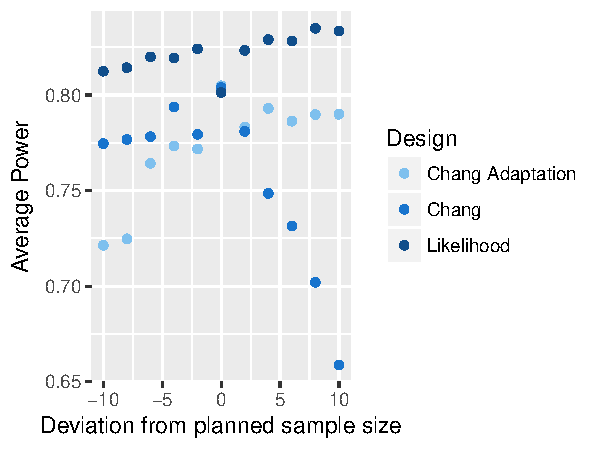
\includegraphics{unnamed-chunk-14-1} }

\end{Schunk}
\end{figure}

\begin{figure}[]
\caption{Monte Carlo Simulation of Average Type I Error Rates of 20 Simon-like Designs when Stage I Sample Size Deviates from Planned for Attained Designs ($n_t^{\ast\ast} = n_t$) Number of Simulations = 500.}
\begin{Schunk}


\centerline{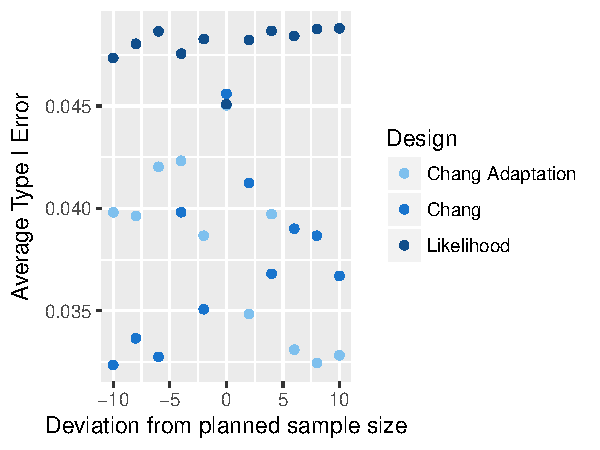
\includegraphics{unnamed-chunk-15-1} }

\end{Schunk}
\end{figure}



%%%%%%%%%%%%%%%%%%%%%%%%%%%%%%%%%%%%%%%%%%%%%%%%%%%%%%%%%%%%%%
%----------------Discussion--------------------------------%
\newpage
\chapter{Discussion and Conclusion}

%%%%%%%%%%%%%%%%%%%%%%%%%%%%%%%%%%%%%%%%%%%%%%%%%%%%%%%%%%%%%%
Deviations from the planned second stage sample size has been better studied than deviations from the planned first stage sample size. Many methods have been proposed on decision rules, and Koyama et al. had introduced a redesign when the first stage sample size is as planned. Because the calculation of a p-value in this case is more straightforward than when stage I differs, there may be less literature proposing redesigns. Here, we focused our investigation and results on deviations from the planned first stage sample size. One argument against redesigning these trials in the first place could be that researchers always have the option to simply wait until stage I sample size is met. In practice, though, some ethical matters may arise that would give the researcher incentive to evaluate the first stage prematurely. For instance, if a new regimen appears to be more beneficial than historical treatments, but statistical requirements prevent new patients from being enrolled until all currently enrolled patients record responses, a researcher may consider this unethical. In this case, $n_1^{\ast\ast} < n_1$ where $n_1^{\ast\ast}$ would be patients who have recorded responses. Having a decision rule for a case such as this would alleviate some discomfort from both the researcher and statistician, though abuse of new decision rules would be discouraged. \\
\indent A numerical study suggested that it may be desireable to redesign trials using the planned total sample size because it better controls type I error for all attained methods and power is closer to the nominal power, on average. Assuming that redesigns use the planned total sample size in the redesign, results from different Simon-like designs were presented.  Chang and the Olson and Koyama methods primarily differ when there are extreme sample size shifts. This is most likely due to the nature of their methods and their primary goals of maintaining type II error spending or probability of early termination. Recommending the use of these designs in practice will depend on the desire of statistical approach of the researcher. If the researcher prefers to use a Frequentist approach in hypothesis testing, it may be recommended that the Olson and Koyama's approach is used because it results in higher average power across deviations. Because it may be of concern that researchers take advantage of the ability to deviate from the planned design, Olson and Koyama's method also penalizes deviation by resulting in a higher probability of early termination when there is underaccrual than Chang's method. \\
\indent We do not consider redesigns when both the first and second stage accrual are not as planned because if one is interested in prespecifying stopping criteria for sample size deviations, the number of combinations needed to be specified in order to prespecify the exact combination that will occur is unreasonable. Though, these attained designs are able to accomodate if this is desired. One advantage to the Likelihood design is that it is able to add cohorts of patients at the end of the second stage if weak evidence is obtained without threatening Frequentist properties such as type I error. Another advantage to the Likelihood approach is that inference is more straightforward because one is not concerned with error rates or p-values. Though we don't consider calculating p-values when stage I differs from planned, it would be complicated if one wished to do so, whereas Likelihood methods would not require this. Likelihood designs are also more generalizable. The Likelihood two-stage approach could be generalized easily to three stages, whereas the Chang designs would not be able to generalize. In this paper, though, we are very much constraining the Likelihood design and not taking full advantage of its natural characteristics. One could simply use a pure Likelihood design and avoid Frequentist issues altogether. \\
\indent A main concern that we have with redesigning trials for unplanned sample sizes is that researchers could take advantage of the these new stopping criteria and stray from the planned design too often. It is for this reason that one may consider adapting Chang's design using a very conservative rule in the first stage and have the probability of early termination under the null always be higher than planned. When deviations are extreme, especially where there is underacrrual, evaluating the trial early would be highly penalized by potentially having a very high probability of early termination. Overall, intentional early or late evaluation of the first stage without sound reason is highly discouraged and will not result in optimal statistical properties. 




%%%%%%%%%%%%%%%%%%%%%%%%%%%%%%%%%%%%%%%%%%%%%%%%%%%%%%%%%%%%%%
%------------------------------------------------%
%%%%%%%%%%%%%%%%%%%%%%%%%%%%%%%%%%%%%%%%%%%%%%%%%%%%%%%%%%%%%%

%%%%%%%%%%%%%%%%%%%%%%%%%%%%%%%%%%%%%%%%%%%%%%%%%%%%%%%%%%%%%%
%-------------- BIBLIOGRAPHY--------------------------------------%
%%%%%%%%%%%%%%%%%%%%%%%%%%%%%%%%%%%%%%%%%%%%%%%%%%%%%%%%%%%%%%


%\bibliographystyle{apacite}
\bibliographystyle{ieeetr}
\bibliography{/Users/mollyolson/Documents/Vanderbilt/Masters_Thesis/ThesisRepo/thesisBib}		

\end{document} 


